\documentclass{beamer}

\usepackage[bulgarian]{babel}
\usepackage{amsfonts,amsmath}
\usepackage{lmodern}
\usepackage[notref,notcite]{showkeys}
\usepackage{graphicx}
\usepackage{wrapfig}
\usepackage{multirow}
\newcommand{\RR}{\mathbb{R}}
\newcommand{\rf}[1]{(\ref{#1})}

\title{Числено решаване на двумерното стационарно парадигматично уравнение на Бузинеск}
\author{докторант: Красимир Ангелов 
\newline \newline научен ръководител: Наталия Кольковска}

\usetheme{default}
\begin{document}

%==================1======================================
\begin{frame}
\titlepage
\end{frame}


%==================2======================================
\begin{frame}
\frametitle{ Едномерното парадигматично уравнение на Бусинеск }
\begin{align}
&u_{tt} - u_{xx} -\beta_1  u_{ttxx} +\beta_2 u_{xxxx} + f(u)_{xx}=0   \quad \text{при} \,  x \in \RR, \, t\in\RR^+,\label{eq1D}
\\ \nonumber &u(x,0)=u_0(x), \, u_t(x,0)=u_1(x)   \quad\text{при} \, x \in \RR,
\\  &u(x) \rightarrow 0,  u(x)_{xx} \rightarrow 0 ,  \quad \text{при} \, x \rightarrow \infty, \label{eq1d1}
\end{align}
Точно решение от тип солитон при $u =\tilde u(x-ct)$:
\begin{align}
\tilde u(x,t:c) = \frac{3}{2} \frac{c^2-1}{\alpha}sech^2 \left( \frac{1}{2}  \sqrt{ \frac{\beta_1 (c^2-1)}{\beta_1 c^2-\beta_2}} (x-c t \sqrt{\frac{\beta_1}{\beta_2}} ) \right)
\end{align}
Солитон е бягаща със скорост $c$ вълна от вида $\phi(x-ct)$, която е локализирана в пространството и при движение запазва формата си. Структурата ѝ се запазва дори след взаимодействие с друг(и) солитон(и).
\end{frame}

%==================3======================================
\begin{frame}
\frametitle{ Двумерното $(x,y) \in \RR^2$ парадигматично уравнение на Бусинеск }
\begin{align}
&u_{tt} - \Delta u -\beta_1  \Delta u_{tt} +\beta_2 \Delta ^2 u + \Delta f(u)=0, \, t\in\RR^+,\label{eq1}
\\
&f(u) = u^2 \nonumber \\  \nonumber &u(x,y,0)=u_0(x,y), \, u_t(x,y,0)=u_1(x,y)  , 
\\  &u(x,y) \rightarrow 0, \,  \Delta u(x,y) \rightarrow 0 ,  \quad \text{при} \sqrt{x^2 + y^2} \rightarrow \infty, \label{eq11} 
\end{align}
\begin{itemize}
  \item Извеждане на {\color{red}стационарно} уравнение чрез полагането $U(x,y-ct)=u(x,y,t)$ в \rf{eq1}
\end{itemize}
\color{red}
\begin{equation}
c^2 (E_1-\beta_1 \Delta) U_{yy} = \Delta U -\beta_2 \Delta^2 U - \Delta f(U)
\end{equation}

\end{frame}

%==================3======================================
\begin{frame}
\frametitle{ Двумерното стационарно парадигматично уравнение на Бусинеск }

\begin{equation}\label{eq2}
c^2 (E_1-\beta_1 \Delta) U_{yy} = \Delta U -\beta_2 \Delta^2 U - \Delta f(U),
\end{equation}
Целта на настоящата работа е
\begin{itemize}
  \item да се намерят числени решения на \rf{eq2} при различни параметри $\beta$ и $c$ с висок ред на апроксимация - 2ри, 4ти и 6ти.
  \item да се намерят числени решения на \rf{eq2} за по-високи скорости близо до допустимия максимум $c \approx \min (\sqrt{\beta_2}/ \sqrt{\beta_1},1)$, $c < \min (\sqrt{\beta_2}/ \sqrt{\beta_1},1)$,
  \item да се построи ново гранично условие за  \rf{eq2}.
\end{itemize}
\end{frame}


%==================55======================================
\begin{frame}
\frametitle{Основни числени инструменти } 
 
\begin{itemize}
  \item дискретизация;
  \item нулево гранично условие;
  \item симетрично гранично условие по абцисата и ординатата при елиптичната задача;
  \item квадратурни формули за пресмятане на двумерни интеграли;
  \item бърз директен метод за обръщане на двумерния оператор на Лаплас.
\end{itemize}

\end{frame}

%==================7.2======================================
\begin{frame}
\frametitle{Основни числени инструменти}

Матриците $\Delta_{h,2,s,x}$ и $\Delta_{h,2,s,y}$ при $p=2$
\[
\frac{1}{h^2}
\begin{bmatrix}
    -2	       & 2        &     \dots   &   \dots        & 0   \\
    1               & -2            &   1           &   0               & \vdots    \\
        0           & \ddots        &    \ddots    &   \ddots       &  0 \\ 
    \vdots       &     0            &  1     	& -2    	   & 1 \\
    0               & \dots          &  \dots         & 1  	   & -2 \\
\end{bmatrix}
\]

Матриците $\Delta_{h,2,x}$ и $\Delta_{h,2,y}$ при $p=2$
\[
\frac{1}{h^2}
\begin{bmatrix}
    -2	       & 1        &     \dots   &   \dots        & 0   \\
    1               & -2            &   1           &   0               & \vdots    \\
        0           & \ddots        &    \ddots    &   \ddots       &  0 \\ 
    \vdots       &     0            &  1     	& -2    	   & 1 \\
    0               & \dots          &  \dots         & 1  	   & -2 \\
\end{bmatrix}
\]
\end{frame}

%==================55======================================

\begin{frame}
\frametitle{Формулировка и числено решение на двумерното стационарно уравнение на Бусинеск - Метод на простата итерация}
\begin{itemize}
  \item Метод на простата итерация - характеристики:
	\begin{itemize}
	% \item смяна на променливите: $x = \sqrt{\beta_1} \bar{x}, \quad y = \sqrt{\beta_1} \bar{y}$;
	  \item начални данни;
	  \item адаптивен метод за контрол на стъпката по времето;
	  \item стоп критерий за итерационната процедура;
	\end{itemize}
  \item Числени резултати;
  \item Сравнение с ``best-fit'' формулите;
  \item Извод на ново асимптотично гранично условие.
\end{itemize}
\end{frame}

%==================5======================================

\begin{frame}
\frametitle{Двумерното стационарно уравнение на Бусинеск}
\framesubtitle{Метод на простата итерация} 
\begin{itemize}
  \item  {\footnotesize J. Choudhury, C.I. Christov,
2D solitary waves of Boussinesq equation, in ISIS International Symposium on Interdisciplinary Science, Natchitoches, October 6-8, 2004, {\it APS Conference Proceedings 755}, Washington, DC, 85-90.}
\end{itemize}
Алгоритмични стъпки:
\begin{itemize}
  \item Въвеждат се две нови функции: $\widehat{v}=v/{\theta} $ и $\widehat{w}=w/{\theta} $, където $v(0,0)=\theta$
\end{itemize}
\begin{equation}\label{eq45}
\begin{split}
 &- (1 - c^2 \beta) \widehat{v}_{yy} -\widehat{v}_{xx} + \beta (1-c^2) \widehat{v} - \alpha \beta \theta \widehat{v}^2 = \widehat{w}, \\
 &- \Delta \widehat{w} =  c^2 \beta \widehat{v}_{xx}.
\end{split}
\end{equation}

\begin{itemize}
  \item Численото решение на системата \rf{eq45} се намира чрез метода на простата итерация като изкуствено се добавят производни по времето както следва:
\end{itemize}
\begin{align}\label{eq5}
\begin{split}
 &\frac {\partial \widehat{v}}{\partial t} - (1 - c^2 \beta) \widehat{v}_{yy} -\widehat{v}_{xx} + \beta (1-c^2) \widehat{v} - \alpha \beta \theta \widehat{v}^2 = \widehat{w}, \\
 &\frac {\partial \widehat{w}}{\partial t} - \Delta \widehat{w} =  c^2 \beta \widehat{v}_{xx}. 
\end{split}
\end{align}
%По този начин стационарната системата от двете уравнения \rf{eq45} се заменя с преходните във времето уравнения дефинирани в \rf{eq5} с условието, че решенията $\widehat{v}$ и $\widehat{w}$ схождат линейно спрямо времето към решенията на \rf{eq45}.



\end{frame}


%==================6======================================
\begin{frame}
\frametitle{Двумерното стационарно уравнение на Бусинеск}
\framesubtitle{Метод на простата итерация} 
Дискретизацията на последното уравнение \rf{eq5} води до следната явна схема:
\begin{equation}\label{eq555}
\begin{split}
\frac {\widehat{v}^{(k+1)}-\widehat{v}^{(k)}}{\tau}- (1-c^2 \beta) \widehat{v}^{(k)}  (\Delta_{h,p,s,y})^T - \quad\quad\quad\;&\\
-\Delta_{h,p,s,x}  \widehat{v}^{(k)}+ \beta (1-c^2 ) \widehat{v}^{(k)} - \beta \theta f(\widehat{v}^{(k)}) &= \widehat{w}^{(k)}, \\
\frac  {\widehat{w}^{(k+1)} -\widehat{w}^{(k)}} {\tau} - \Delta_{h,p,s,x}  \widehat{w}^{(k)} - \widehat{w}^{(k)}  (\Delta_{h,p,s,y})^T &=  c^2 \beta \Delta_{h,p,s,x}  \widehat{v}^{(k)}.
\end{split}
\end{equation}

Стойността на $\theta$ се намира използвайки следната зависимост
\begin{equation}\label{eqtheta}
\theta = \frac{ (1-c^2 \beta) \widehat{v}_{yy} + \widehat{v}_{xx} - \beta (1-c^2) \widehat{v} +\widehat{w}}{\alpha \beta \widehat{v}^2 } |_{x=0,y=0}.
\end{equation}
\end{frame}


%==================13=====================================
\begin{frame}
\frametitle{Ред на сходимост при Тест 1 - $\beta = 3$, $c=0.45$}

\begin{table}[ht]
\centering
		\begin{tabular}{||c|l|ll|ll||}
			\hline
			\hline
             & $h$  &  	$\Vert \bar{ E_i} \Vert_{L_2}$ 	& сход.	& $\Vert \bar{ E_i} \Vert_{L_\infty}$  		&сход.   \\
   					\hline 
					\hline 
$\beta = 3$   	&0.2    										&            &            &           &   \\
      c=0.45 	&0.1    & 0.014232  						&            & 0.016732 			&   \\
   $O(h^2)$     &0.05   & 0.003238  						&2.14  & 0.003997					& 2.07 \\
\hline 
$\beta = 3$   	&0.2   &            &            &             &    \\
      $c=0.45 $ &0.1   &   0.001758   &           &  0.002499  &   \\
       $O(h^4)$	&0.05  &  0.000114 & 3.95    & 0.000168  & 3.90  \\
\hline
$\beta = 3$   	&0.2   &            &        &                  &      \\
   $c=0.45$   	&0.1   &  0.005038 &           & 0.012462       &       \\
     $O(h^6)$	&0.05  &  0.000094  & 5.74  &  0.000323 & 5.27         \\
			\hline
			\hline 
		\end{tabular}
		\caption{Ред на сходимост при Метода на простата итерация с апроксимации $O(h^{2})$, $O(h^{4})$ и $O(h^{6})$ за Тест  1. Грешките $\bar{ E_i}$ са пресметнати в $L_2$ и $L_\infty$ норми.}
\label{tab:aA}
\end{table}

\end{frame}


%==================14=====================================
\begin{frame}
\frametitle{Двумерното стационарно уравнение на Бусинеск}
\framesubtitle{Ред на сходимост при Тест 2 - $\beta = 1$, $c=0.9$}

\begin{table}[ht]
\centering
		\begin{tabular}{||c|l|ll|ll||}
			\hline
			\hline
             & $h$  &  	$\Vert \bar{ E_i} \Vert_{L_2}$ 	& сход.	& $\Vert \bar{ E_i}\Vert_{L_\infty}$  		&сход.   \\
   					\hline 					
			\hline 	
$\beta = 1$   	&0.4   &             &           &                & \\
     $c=0.9$     &0.2   &  0.043898  &             & 0.017906      &    \\
     $O(h^2)$	&0.1  & 0.009999 & 2.13       & 0.004348      & 2.04  \\
\hline 	
 $\beta = 1$   	&0.4  &            &               &               &     \\
     $c=0.9$  	&0.2   & 0.006309  &              & 0.002965      &        \\
     $O(h^4)$	&0.1  &  0.000432 &3.87        & 0.000200 &  3.89        \\
    \hline
 $\beta = 1$	&0.4   &             &        &               &        \\
   $ c=0.9$  	&0.2   &  0.001423  &        & 0.000728      &       \\
       $O(h^6)$	&0.1  &   0.000121 &3.56  & 0.000015 &   5.57       \\
	   \hline
			\hline 
		\end{tabular}
		\caption{Ред на сходимост при Метода на простата итерация с апроксимации $O(h^{2})$, $O(h^{4})$ и $O(h^{6})$ и Тест 2. Грешките $\bar{ E_i}$ са пресметнати в $L_2$ и $L_\infty$ норми.}
\label{tab:aB}
\end{table}

\end{frame}

%==================16=====================================
\begin{frame}
\frametitle{Двумерното стационарно уравнение на Бусинеск}
\framesubtitle{Форма на решението}
\begin{figure}[ht]
	\begin{minipage}[b]{0.45\linewidth}
		\raggedleft
		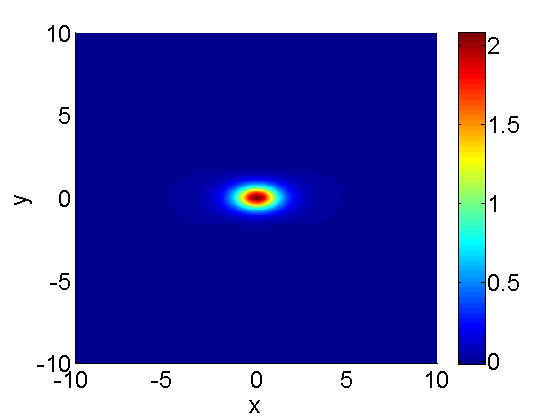
\includegraphics[width=\linewidth]{../Thesis/SolutionView/ChristovIC_30_bt3_c045_topview.png}
	\end{minipage}
	\begin{minipage}[b]{0.45\linewidth}
		\raggedright
		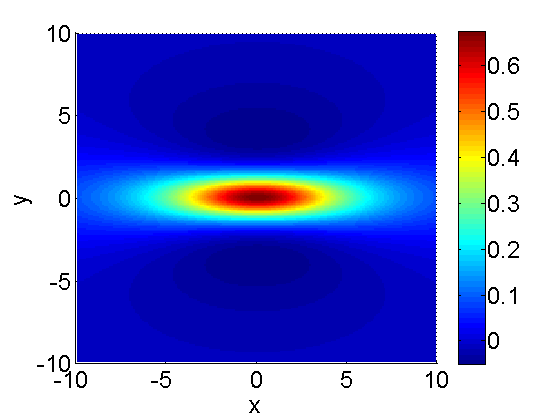
\includegraphics[width=\linewidth]{../Thesis/SolutionView/ChristovIC_128_bt1_c090_topview.png}
	\end{minipage}
	\begin{minipage}[b]{0.45\linewidth}
		 \raggedleft
		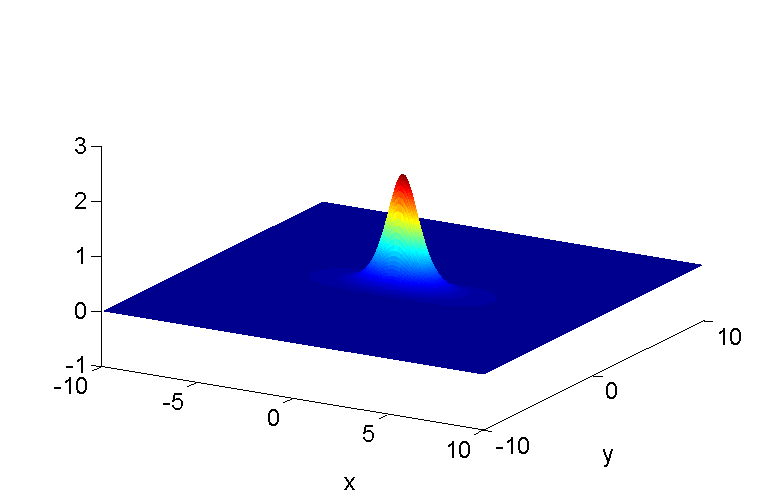
\includegraphics[width=\linewidth]{../Thesis/SolutionView/ChristovIC_30_bt3_c045_prpview.png}		
		\centerline{$\beta = 3$, $c = 0.45$ }
	\end{minipage}
	\begin{minipage}[b]{0.45\linewidth}
		 \raggedright
		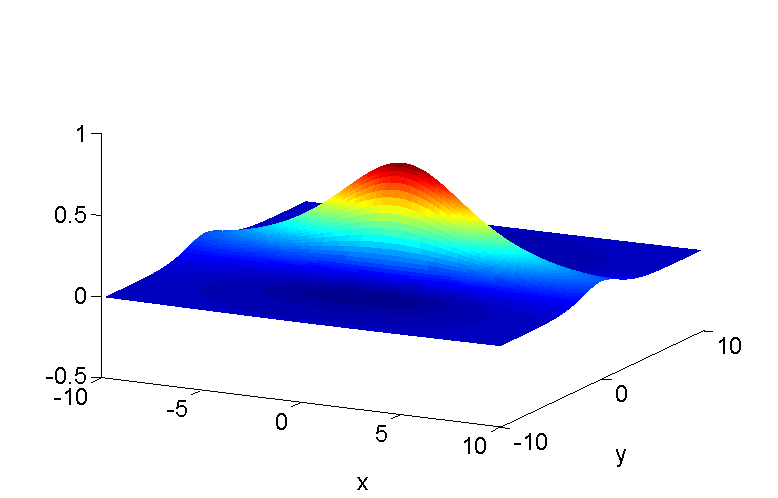
\includegraphics[width=\linewidth]{../Thesis/SolutionView/ChristovIC_128_bt1_c090_prpview.png}
		\centerline{$\beta = 1$, $c = 0.9$}
	\end{minipage}
	\caption{2Д и 3Д профили на численото решение $\widehat v$ от \rf{eqtheta} и \rf{eq555}.}
	\label{fig:solutions}
\end{figure}

\end{frame}

%==================17=====================================
\begin{frame}
\frametitle{Двумерното стационарно уравнение на Бусинеск}
\framesubtitle{Сравнение с ``best-fit'' формулите}

Нека $D^*_{\kappa}$ да дефинира процентната разликата между двете решения  ``Метода на простата итерация'' $v$ и ``best-fit'' $v^*$ в ${L_2 }$ и ${L_\infty}$ норми, върху цялата област $\omega_h$:
\begin{equation}\label{diffvv}
D^*_{\kappa} := 100 \times \frac{\Vert v^*-v \Vert_{\kappa} }{ \Vert v \Vert_{\kappa} }.
\end{equation}
\end{frame}

%==================18=====================================
\begin{frame}
\frametitle{Двумерното стационарно уравнение на Бусинеск}
\framesubtitle{Сравнение с ``best-fit'' формулите}
\begin{table}[ht]
\centering
\begin{tabular}{|l|c|l l|l l|}
\hline 
\hline 
$\beta$	& c 	& $\|v^*-v \|_{L_2 }$ & $\|v^*-v \|_{L_\infty }$  	& $D^*_{L_2}$	& $D^*_{L_\infty }$	\\
\hline 
1& 		0.1	&	1.4772e-01 		& 	8.1024e-03 				& 2.7\%			& 1.7\%		\\
\hline 
1& 		0.3 	&	1.4310e-01 		& 	8.7770e-03				& 2.7\%			& 1.9\%		\\
\hline 
1& 		0.5 	&	1.6934e-01 		& 	1.3332e-02				& 3.5\%			& 3.3\%		\\
\hline 
1& 		0.7 	&	5.8673e-01		& 	5.1122e-02				& 14.8\%		& 16.2\%	\\
\hline 
1& 		0.9	&	2.1599e+0 		& 	1.6439e-01				& 93.1\%		& 121.2\%	\\
\hline 
\hline 
\end{tabular}
\caption{Разликите между числено решение $v$ получено с ``Метода на простата итерация'' и ``best-fit'' формулите $v^*$ при $\beta=1$ и $c=0.1, 0.3, 0.5, 0.7, 0.9$.}
\label{tab:diff-beta1}
\end{table}

\end{frame}

%==================19=====================================
\begin{frame}
\frametitle{Двумерното стационарно уравнение на Бусинеск}
\framesubtitle{Сравнение с ``best-fit'' формулите}
\begin{table}
\centering
\begin{tabular}{|l|c|l l| c|l|c|l l|}
\hline 
\hline 
$\beta$	& c 	& $\|v^*-v \|_{L_2 }$ & $\|v^*-v \|_{L_\infty }$  	& $D^*_{L_2}$	& $D^*_{L_\infty }$	\\
\hline 
1& 		0.17&	1.4704e-01 		& 	8.3793e-03 				& 2.7\%			& 1.8\%		\\
\hline 
2& 		0.17&	1.2688e-01 		& 	9.0013e-03				& 3.3\%			& 1.9\%		\\
\hline 
3& 		0.17&	1.3803e-01 		& 	1.3134e-02				& 4.4\%			& 2.8\%		\\
\hline 
4& 		0.17&	 1.5240e-01 		& 	1.7228e-02				& 5.7\%			& 3.7\%		\\
\hline 
5& 		0.17&	1.6720e-01 		& 	2.1844e-02				& 7.0\%			& 4.6\%		\\
\hline 
\hline 
\end{tabular}
\caption{Разликите между числено решение $v$ получено с ``Метода на простата итерация'' и ``best-fit'' формулите $v^*$ от \cite{Ch2011} при $\beta=1, 2, 3, 4, 5$ и $c=0.17$.}
\label{tab:diff-c017}
\end{table}
\end{frame}

%==================20=====================================
\begin{frame}
\frametitle{Двумерното стационарно уравнение на Бусинеск}
\framesubtitle{Извод на ново асимптотично гранично условие}

\begin{itemize}
 {\footnotesize \item  C.I. Christov,
Numerical implementation of the asymptotic boundary conditions for steadily propagating 2D solitons of Boussinesq type equations,
{\it Mathematics and Computers in Simulation}, \textbf{82} (2012), 1079-1092.}
\begin{equation}
v(x,y) = v(r) ~ \frac{C_u}{r^2}, \quad r>>1
\end{equation}
  \item ново асимптотично гранично условие
\begin{equation}\label{bndK}
\tilde v(x,y) = \mu_v \frac{ (1-c^2)x^2 - y^2}{ ((1-c^2)x^2 - y^2)^2}, \quad x^2 + y^2 >> 1.
\end{equation}
\end{itemize}
 

\end{frame}

%==================21=====================================
\begin{frame}
\frametitle{Двумерното стационарно уравнение на Бусинеск}
\framesubtitle{Асимптотично поведение на членовете в уравнението}
\begin{figure}
	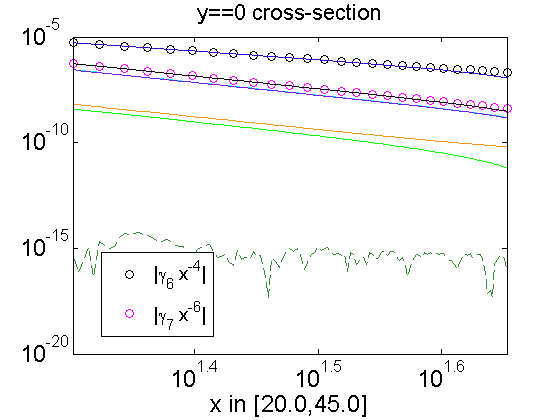
\includegraphics[width=0.8\linewidth]{../Thesis/AssymptForEachTerm/c017_bt1_5/ChristovIC_AlongX_50_ZB2_bt1_c017_h020_O(h^6).png}
	\caption{Решението е получено с ``Метода на простата итерация'' и нулево гранично условие, $\boldsymbol{c=0.17}$ и $\boldsymbol{\beta = 1}$. }
	\label{fig:assympt_c017bt11}
\end{figure}

\end{frame}

%==================22=====================================
\begin{frame}
\frametitle{Двумерното стационарно уравнение на Бусинеск}
\framesubtitle{Асимптотично поведение на членовете в уравнението}
\begin{figure}
	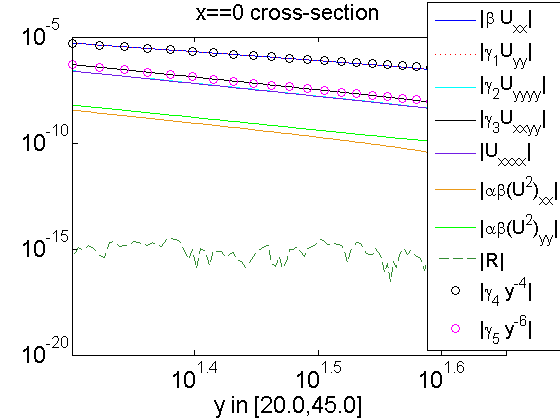
\includegraphics[width=0.8\linewidth]{../Thesis/AssymptForEachTerm/c017_bt1_5/ChristovIC_AlongY_50_ZB2_bt1_c017_h020_O(h^6).png}
	\caption{ Решението е получено с ``Метода на простата итерация'' и нулево гранично условие, $\boldsymbol{c=0.17}$ и $\boldsymbol{\beta = 1}$. }
	\label{fig:assympt_c017bt12}
\end{figure}


\end{frame}

%==================23=====================================
\begin{frame}
\frametitle{Двумерното стационарно уравнение на Бусинеск}
\framesubtitle{Асимптотично поведение на членовете в уравнението}
Представените фигури в предишната част показват, че асимптотиката на членовете с производни от четвърти ред и нелинейните такива с производни от втори ред
\begin{equation}\label{outliers}
- v_{xxxx}, \;  - (2-\beta c^2)v_{xxyy},  \;  - (1-\beta c^2)v_{yyyy}, \;  - \alpha \beta (v^2)_{xx}, \; - \alpha \beta (v^2)_{yy}
\end{equation}
e $O(r^{-6})$, а за останалите от втори ред
$$
\beta v_{xx}, \; \beta (1-c^2) v_{yy}
$$
асимптотиката е $O(r^{-4})$. Това дава основание да пренебрегнем членовете описани в \rf{outliers} от уравнение \rf{eq3} и да търсим точно решение на останалата част.
\end{frame}

%==================24=====================================
\begin{frame}
\frametitle{Двумерното стационарно уравнение на Бусинеск}
\framesubtitle{Извод на ново гранично условие}
Така за големи стойности на $r$, пренебрегвайки частите с по-нисък порядък $O(r^{-6})$, остават два водещи члена:
\begin{equation}\label{asymptEq}
\beta \tilde v_{xx} + \beta (1-c^2) \tilde v_{yy} =0, \quad \tilde v(x,y) \approx \frac{1}{x^2 + y^2}, \quad x^2 + y^2 >>1,
\end{equation} 
взимайки предвид факта, че функцията $v(r)$ има асимптотика $O(r^{-2})$. Следният клас от функции се явява решение на уравнението:
\begin{equation}\label{bndK}
\tilde v(x,y) = \mu_v \frac{ (1-c^2)x^2 - y^2}{ ((1-c^2)x^2 - y^2)^2}, \quad x^2 + y^2 >> 1.
\end{equation}
\end{frame}

%==================5======================================


\begin{frame}
\frametitle{Формулировка и числено решение на двумерното Парадигматично уравнение на Бусинеск}
 
\begin{itemize}
  \item смяна на променливите:
$
x = \sqrt{\beta_1} \bar{x}, \quad y = \sqrt{\beta_1} \bar{y}, \quad t = \sqrt{\beta_1} \bar{t};
$
  \item Консервативна схема;
  \item метод на Тейлор в комбинация с метод на правите;
  \item Числени резултати за двата метода:
  \begin{itemize}
	  \item ред на сходимост по правилото на Рунге;  
	  \item сравнение между метода на Тейлор и Консервативната схема за енергията, масата и формата;
	  \item резултати за формата и максимума при по-голям времеви интервал [0, 30].
	\end{itemize}
  \item Числен тест за хиперболичната задача при параметри $\beta = 3$ и $c=0.3$.
\end{itemize}

\end{frame}

%---------- frame 08 ----------------
\begin{frame}
\frametitle{Масата и енергията за непрекъснатата задача }
\begin{itemize}
\item {\footnotesize Christov C., An energy-consistent dispersive shallow-water model, Wave Motion;}
\item {\footnotesize Todorov M., Nonlinear Waves: Theory, computer simulation, experiment, Two-dimensional Boussinesq equation. Boussinesq paradigm and soliton solutions.}
\end{itemize}
Масата:
\begin{equation}\label{intM}
M(u(x,y,t))=\int_{\RR^2} u(x,y,t)dx dy = const.
\end{equation}

Енергията:
\begin{align}\label{ex-en}
E(u(x,y,t)) = &\int_{R^2} u_t \left((A^{-1}+E)u_t\right) dxdy+
\beta \int_{R^2} u^2 dxdy \nonumber\\
+& \int_{R^2}u \left(A u\right) dxdy
-\frac{2 \alpha \beta}{3} \int_{R^2} u^3 dxdy =const.
\end{align}
където $Au=-\Delta u$ и $Au,-\Delta u$ и $u$ са непрекъснати функции.

\end{frame}

%------------------------- frame 14 -----------------------------------------

\begin{frame}
\frametitle{Метод на Тейлор и метод на правите за ПУБ}
\begin{center}\vspace{0.25cm}
	\begin{minipage}[b]{0.45\linewidth}
		 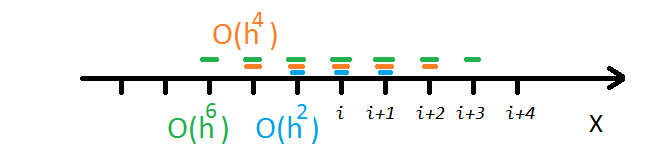
\includegraphics[width=\linewidth]{../amitans/figures/FDS.png}
	\end{minipage}	
\end{center}
Нека $u_{i,j}(t)$ е апроксимацията на $u(x_i, y_j, t)$ в точка от мрежата $(x_i, y_j)$.
\\
Нека $\Delta_{h,p} u_{i,j}$ е диференчния оператор, който апроксимира $\Delta u$ с грешкa $O(|h|^p)$ (p=2, 4, 6).
\\
%here99
От  се получава следната система от ОДУ:
\begin{equation}\label{DiscreteEq}
\beta (I-\Delta_{h,p}) \frac{\partial^2 u}{\partial t^2}(x_i, y_j, t)=
 (\Delta_{h,p} - \Delta_{h,p}^2) u_{i, j}(t) + \Delta_{h,p} ( ( u_{i, j}(t) )^2 )
\end{equation}
за $i = 0..N_1$ и $j=0..N_2$. За всяко ОДУ от системата е направено развитие в ред на Тейлор:
\begin{align} \label{TSe}
u(x_i, y_j, t+\tau) = u(x_i, y_j, t) + \tau \frac{ \partial u }{ \partial t }(x_i, y_j, t)  + ... 
%\nonumber
%\\
\frac{ \tau^p }{ p! } \frac{ \partial^p u }{ \partial t^p }(x_i, y_j, t) + O(\tau^{p+1})
\end{align}

\end{frame}

%==================30=====================================
\begin{frame}
\frametitle{Заключение}

\begin{itemize}
  \item Намерено е числено решение на стационарното уравнение на Бусинеск с висок ред на апроксимация $O(h^4)$ и $O(h^6)$
  \item така се намират нови числени решения за произволни параметри $\beta, c$ с условието, че $c < \min (1/ \sqrt{\beta},1)$
  \item направени са сравнения с ``best-fit'' формулите на проф. Христов,
  \item изведено е ново гранично условие
\end{itemize}

Това ни дава достатъчно знания, за да преминем към изследване на хиперболичната задача \rf{eq1} - \rf{eq11}
\end{frame}

\end{document}